\subsection{Comparison of Models}

The purpose of this work serves to provide recommendations for developing a wireless network intrusion detection system; however, evaluating the performances of the models poses a challenge when determining the 'best' model for each algorithm. Challenges arise when multiple metrics and performance indicators are to be compared. The analysis focused on achieving a balance between avoiding false positives (instances where normal traffic is marked as malicious) and false negatives (instances of malicious traffic marked as normal). The aim was to identify a model capable of distinguishing between the six attack classes and avoiding as many false negatives and positives as possible. The following sections compare the three 'best' identified models from the following models: Random Forest, XGBoost and Multi-Layer Perceptron (MLP).

\subsubsection*{Random Forest}

During experimentation, several Random Forest models were trained, and attempts were made to search through a series of parameters; using the evaluation metrics defined previously, Model ID 1 displayed robust and consistent performance during CV and testing. It achieved an AUC of 99.99, F1 of 99.66, Precision of 99.66, Recall of 99.67 and Accuracy of 99.67 on the test set, indicating that it was able to correctly classify the six attack classes with a high degree of accuracy. The model's confusion matrix shows a good balance between FP and FNs on majority classes; whilst it struggled slightly on Botnet and SSH, the total misclassification remained relatively low. \ref{tab:rf_class_report}, \ref{fig:rf_model1_cm} and \ref{fig:rf_model1_fi} show the Classification, Confusion Matrix and Feature Importances for the model.

\begin{table}[htbp]
  \centering
  \caption{RF Model 1 - Classification Report}
  \label{tab:rf_class_report}
    \begin{tabular}{lcccc}
    \toprule
    Class & Precision & Recall & F1-Score & Support \\
    \midrule
    Botnet & 0.95 & {\color{red}\bfseries 0.77} & {\color{red}\bfseries 0.85} & 17060 \\
    Malware & {\color{red}\bfseries 0.89} & 0.82 & 0.86 & 39476 \\
    Normal & 1.00 & 1.00 & 1.00 & 4572206 \\
    SQL Injection & 0.93 & 0.86 & 0.89 & 789 \\
    SSDP & 1.00 & 1.00 & 1.00 & 1649955 \\
    SSH & 0.94 & 0.79 & 0.86 & 3565 \\
    Website Spoofing & 0.99 & 0.98 & 0.98 & 121533 \\
    \midrule
    Accuracy & & & 1.00 & 6404584 \\
    Macro Avg & 0.96 & 0.89 & 0.92 & 6404584 \\
    Weighted Avg & 1.00 & 1.00 & 1.00 & 6404584 \\
    \bottomrule
    \end{tabular}
\end{table}

\begin{figure}[H]
    \centering
	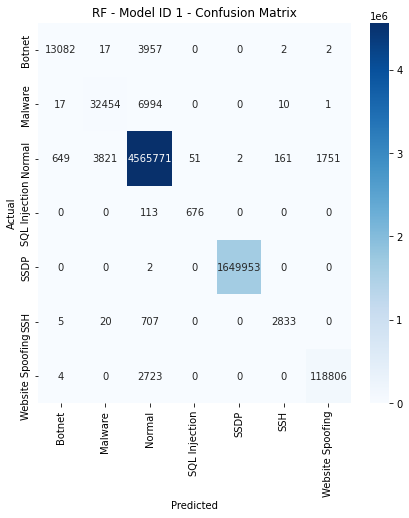
\includegraphics[width=0.8\textwidth]{Appendices/Images/RF/Model1/RF_Model1_CM.png}
	\caption{RF Model 1 - CM}
  	\label{fig:rf_model1_cm}
\end{figure}

\begin{figure}[H]
    \centering
	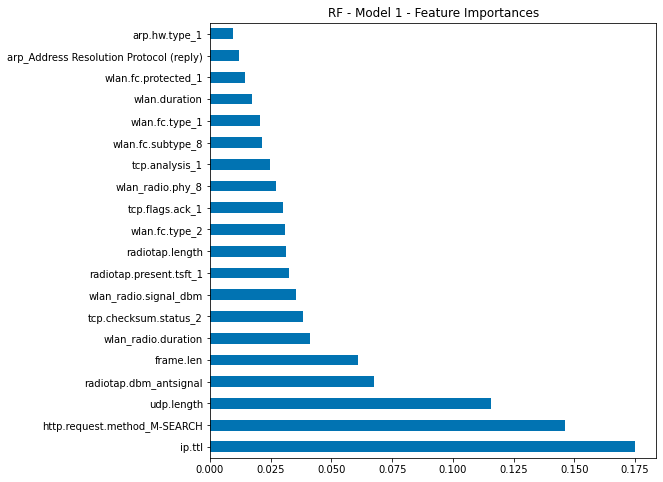
\includegraphics[width=\textwidth]{Appendices/Images/RF/Model1/RF_Model1_FI.png}
	\caption{RF Model 1 - FI}
  	\label{fig:rf_model1_fi}
\end{figure}


\subsubsection*{XGBoost}

Comparing all 11 models trained on the XGBoost Classifier, Model 10 achieved superiority with an AUC of 99.99 (rounding to 100), F1 of 99.65, Precision of 99.65, Recall of 99.66 and Accuracy of 99.66 across the test set and similar during Cross Validated training. It was considered to be the best-performing model from the selection and proved to be robust and efficient. \ref{tab:xgb_class_report}, \ref{fig:xgb_model10_cm} and \ref{fig:xgb_model10_fi} show the Classification, Confusion Matrix and Feature Importances for the model.


\begin{table}[htbp]
  \centering
  \caption{XGBoost Model 10 - Classification Report}
  \label{tab:xgb_class_report}
    \begin{tabular}{lcccc}
    \toprule
    Class & Precision & Recall & F1-Score & Support \\
    \midrule
    Botnet & 0.96 & 0.75 & {\color{red}\bfseries 0.84} & 17060 \\
    Malware & {\color{red}\bfseries 0.89} & 0.82 & 0.85 & 39476 \\
    Normal & 1.00 & 1.00 & 1.00 & 4572206 \\
    SQL Injection & 0.94 & 0.89 & {\color{red}\bfseries 0.91} & 789 \\
    SSDP & 1.00 & 1.00 & 1.00 & 1649955 \\
    SSH & 0.92 & {\color{red}\bfseries 0.78} & 0.85 & 3565 \\
    Website Spoofing & 0.99 & 0.97 & 0.98 & 121533 \\
    \midrule
    Accuracy & & & 0.99 & 6404584 \\
    Macro Avg & 0.83 & 0.73 & 0.80 & 6404584 \\
    Weighted Avg & 0.99 & 0.99 & 0.99 & 6404584 \\
    \bottomrule
    \end{tabular}
\end{table}

\begin{figure}[H]
	\centering
	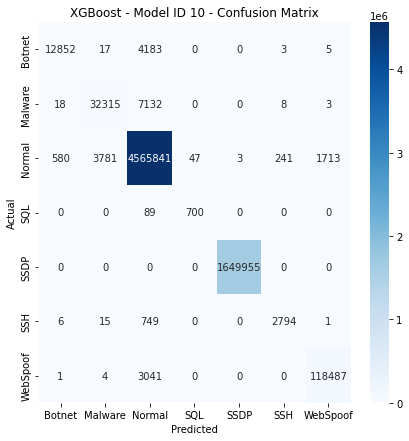
\includegraphics[width=0.8\textwidth]{Appendices/Images/XGB/Model10/XGB_Model10_CM.png}
	\caption{XGBoost Model 10 - CM}
  	\label{fig:xgb_model10_cm}
\end{figure}

\begin{figure}[H]
	\centering
	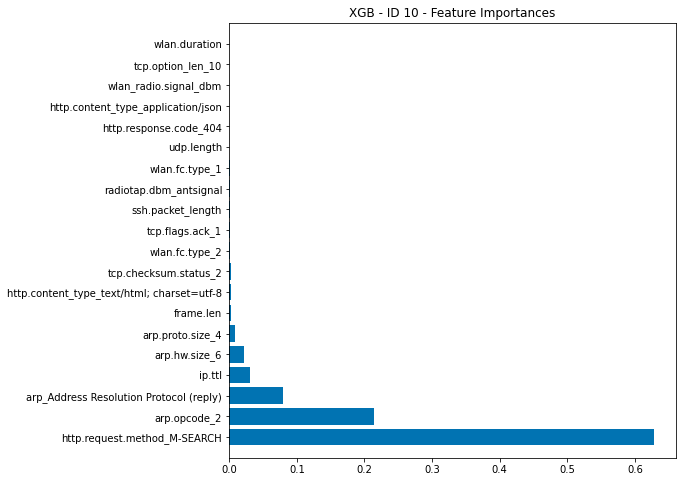
\includegraphics[width=\textwidth]{Appendices/Images/XGB/Model10/XGB_Model10_FI.png}
	\caption{XGBoost Model 10 - FI}
  	\label{fig:xgb_model10_fi}
\end{figure}


% MLP
\subsubsection*{MLP}

Out of all models trained, model 4 showed strong performance overall, with a good proportion of instances from classes Botnet, Malware, Normal and SSDP being accurately classified. While the model struggles with SQL Injection and SSH with poor recall and F1 scores, this was expected given the imbalance in the dataset. Metrics were consistent across S-CV and the test set, indicating that the MLP model was not overfitting the training data and generalising well on new unseen data. Refer to \ref{tab:mlp_class_report} and \ref{fig:mlp_model4_cm} for the Classification Report and Confusion Matrix for the model. The lowest scores per column are denoted in red. Figure \ref{fig:mlp_model4_folds} shows the best and worst fold between the ten folds in training. In the lowest fold, the model starts to overfit on the training data after epoch 2, and in two consecutive folds with no improvements, early stopping interrupted the fold.

\begin{table}[htbp]
  \centering
  \caption{MLP Model 4 - Classification Report}
  \label{tab:mlp_class_report}
    \begin{tabular}{lcccc}
    \toprule
    Class & Precision & Recall & F1-Score & Support \\
    \midrule
    Botnet & 0.94 & 0.61 & 0.74 & 17060 \\
    Malware & 0.89 & 0.72 & 0.80 & 39476 \\
    Normal & 0.99 & 1.00 & 1.00 & 4572206 \\
    SQL Injection & 0.99 & {\color{red}\bfseries 0.37} & {\color{red}\bfseries 0.54} & 789 \\
    SSDP & 1.00 & 1.00 & 1.00 & 1649955 \\
    SSH & {\color{red}\bfseries 0.83} & 0.48 & 0.60 & 3565 \\
    Website Spoofing & 1.00 & 0.92 & 0.95 & 121533 \\
    \midrule
    Accuracy & & & 0.99 & 6404584 \\
    Macro Avg & 0.83 & 0.73 & 0.80 & 6404584 \\
    Weighted Avg & 0.99 & 0.99 & 0.99 & 6404584 \\
    \bottomrule
    \end{tabular}
\end{table}

\begin{figure}[H]
    \centering
	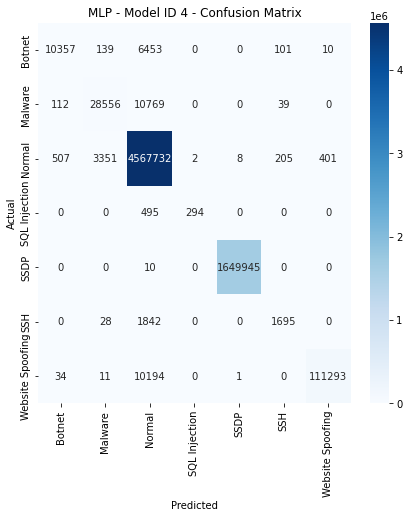
\includegraphics[width=0.8\textwidth]{Appendices/Images/MLP/Model4/MLP_Model4_CM.png}
	\caption{MLP Model 4 - CM}
  	\label{fig:mlp_model4_cm}
\end{figure}


\begin{figure}[H]
    \centering
    \begin{subfigure}{0.45\textwidth}
        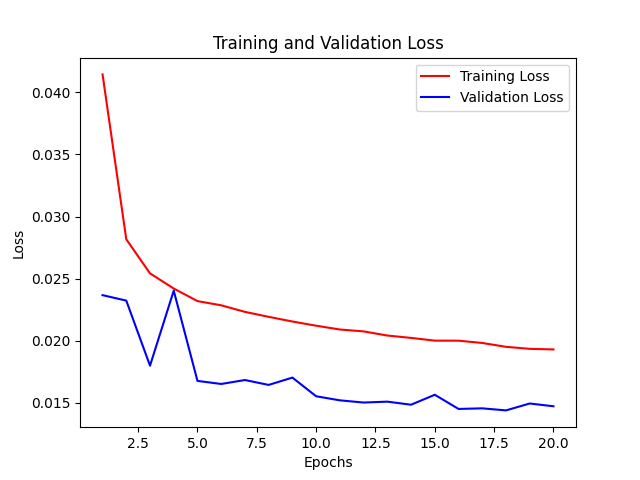
\includegraphics[width=\textwidth]{Appendices/Images/MLP/Model4/MLP_Fold_4_Loss.png}
        \caption{MLP Model 4 - Best Fold}
        \label{fig:mlp_model4_best_fold}
    \end{subfigure}
    \hfill
    \begin{subfigure}{0.45\textwidth}
        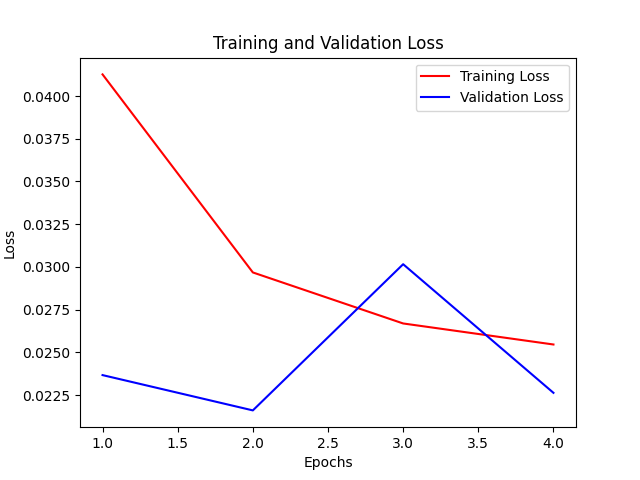
\includegraphics[width=\textwidth]{Appendices/Images/MLP/Model4/MLP_Fold_6_Loss.png}
        \caption{MLP Model 4 - Worst Fold}
        \label{fig:mlp_model4_worst_fold}
    \end{subfigure}
    \caption{MLP Model 4 - Best and Worst Folds}
    \label{fig:mlp_model4_folds}
\end{figure}

\begin{table}[h]
\centering
\caption{Best Models}
\label{tab:ml-metrics}
\begin{tabular}{|l|l|l|l|l|l|l|l|}
\hline
\textbf{Model} & \textbf{AUC} & \textbf{F1} & \textbf{Precision} & \textbf{Recall} & \textbf{Accuracy}  \\ \hline
Random Forest & 99.99 & 99.66 & 99.66 & 99.67 & 99.67 \\ \hline
XGBoost & 99.99 & 99.65 & 99.65 & 99.66 & 99.66 \\ \hline
MLP & 99.94 & 99.42 & 99.44 & 99.46 & 99.46 \\ \hline
\end{tabular}
\end{table}

\begin{figure}[H]
    \centering
	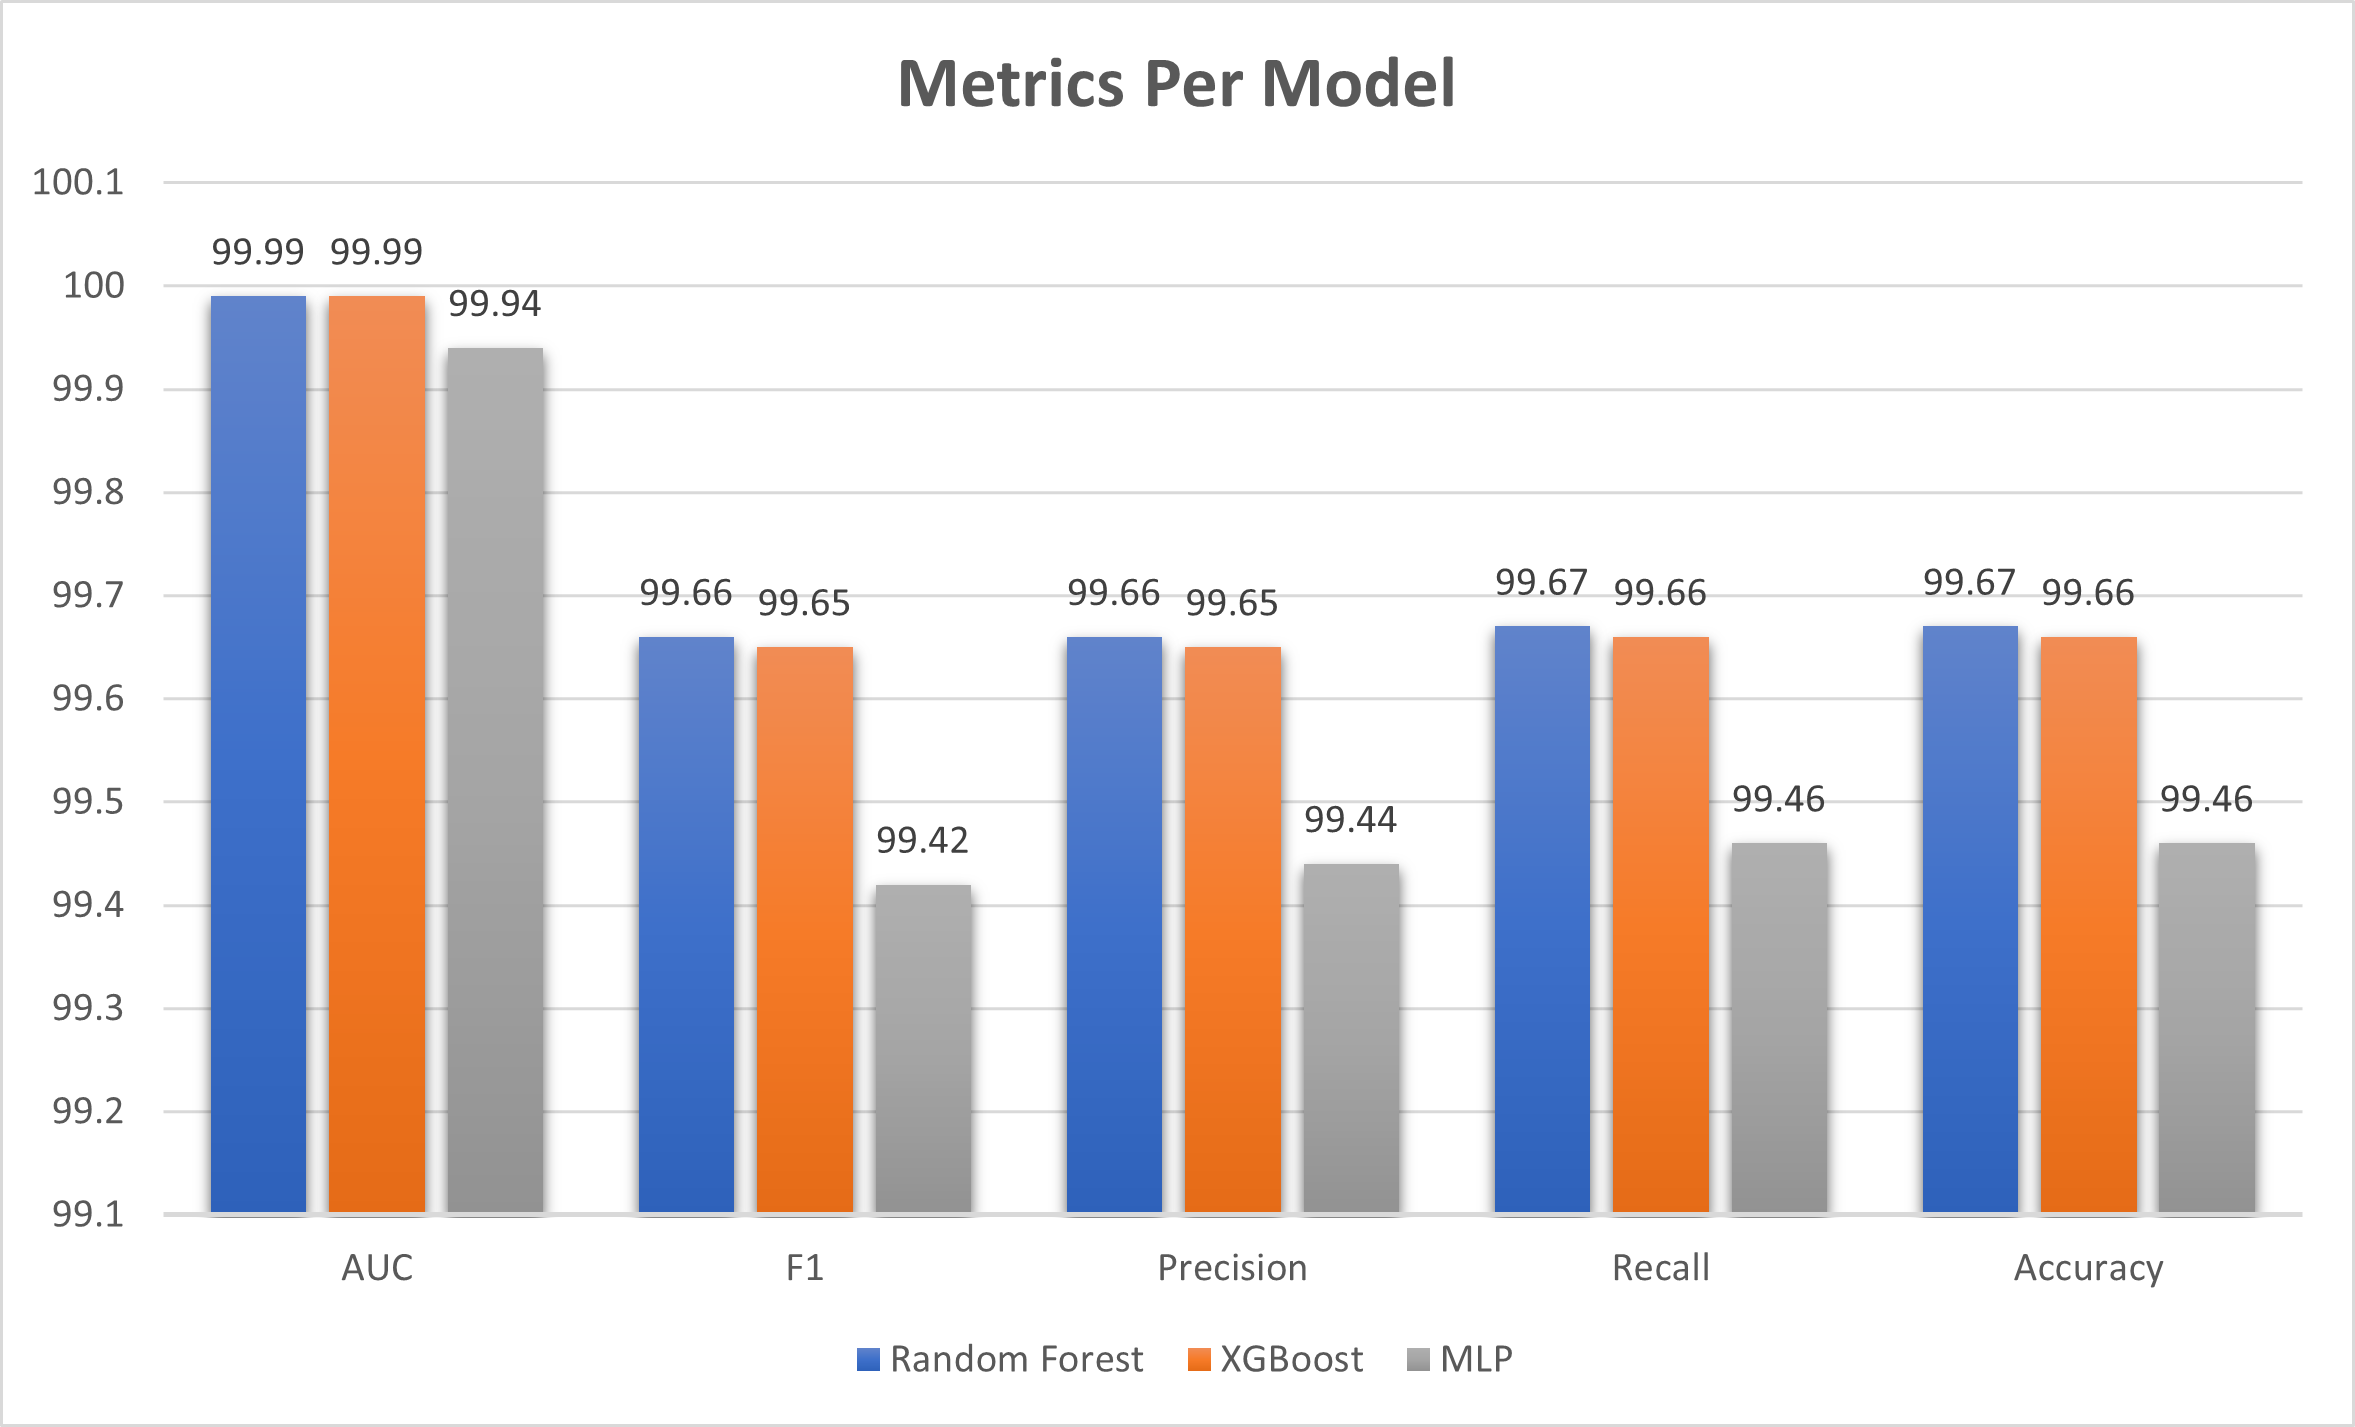
\includegraphics[width=\textwidth]{Appendices/Images/Metrics.png}
	\caption{Models Grouped By Metric}
  	\label{fig:model_metrics_graph}
\end{figure}
\begin{figure}[H]
    \centering
	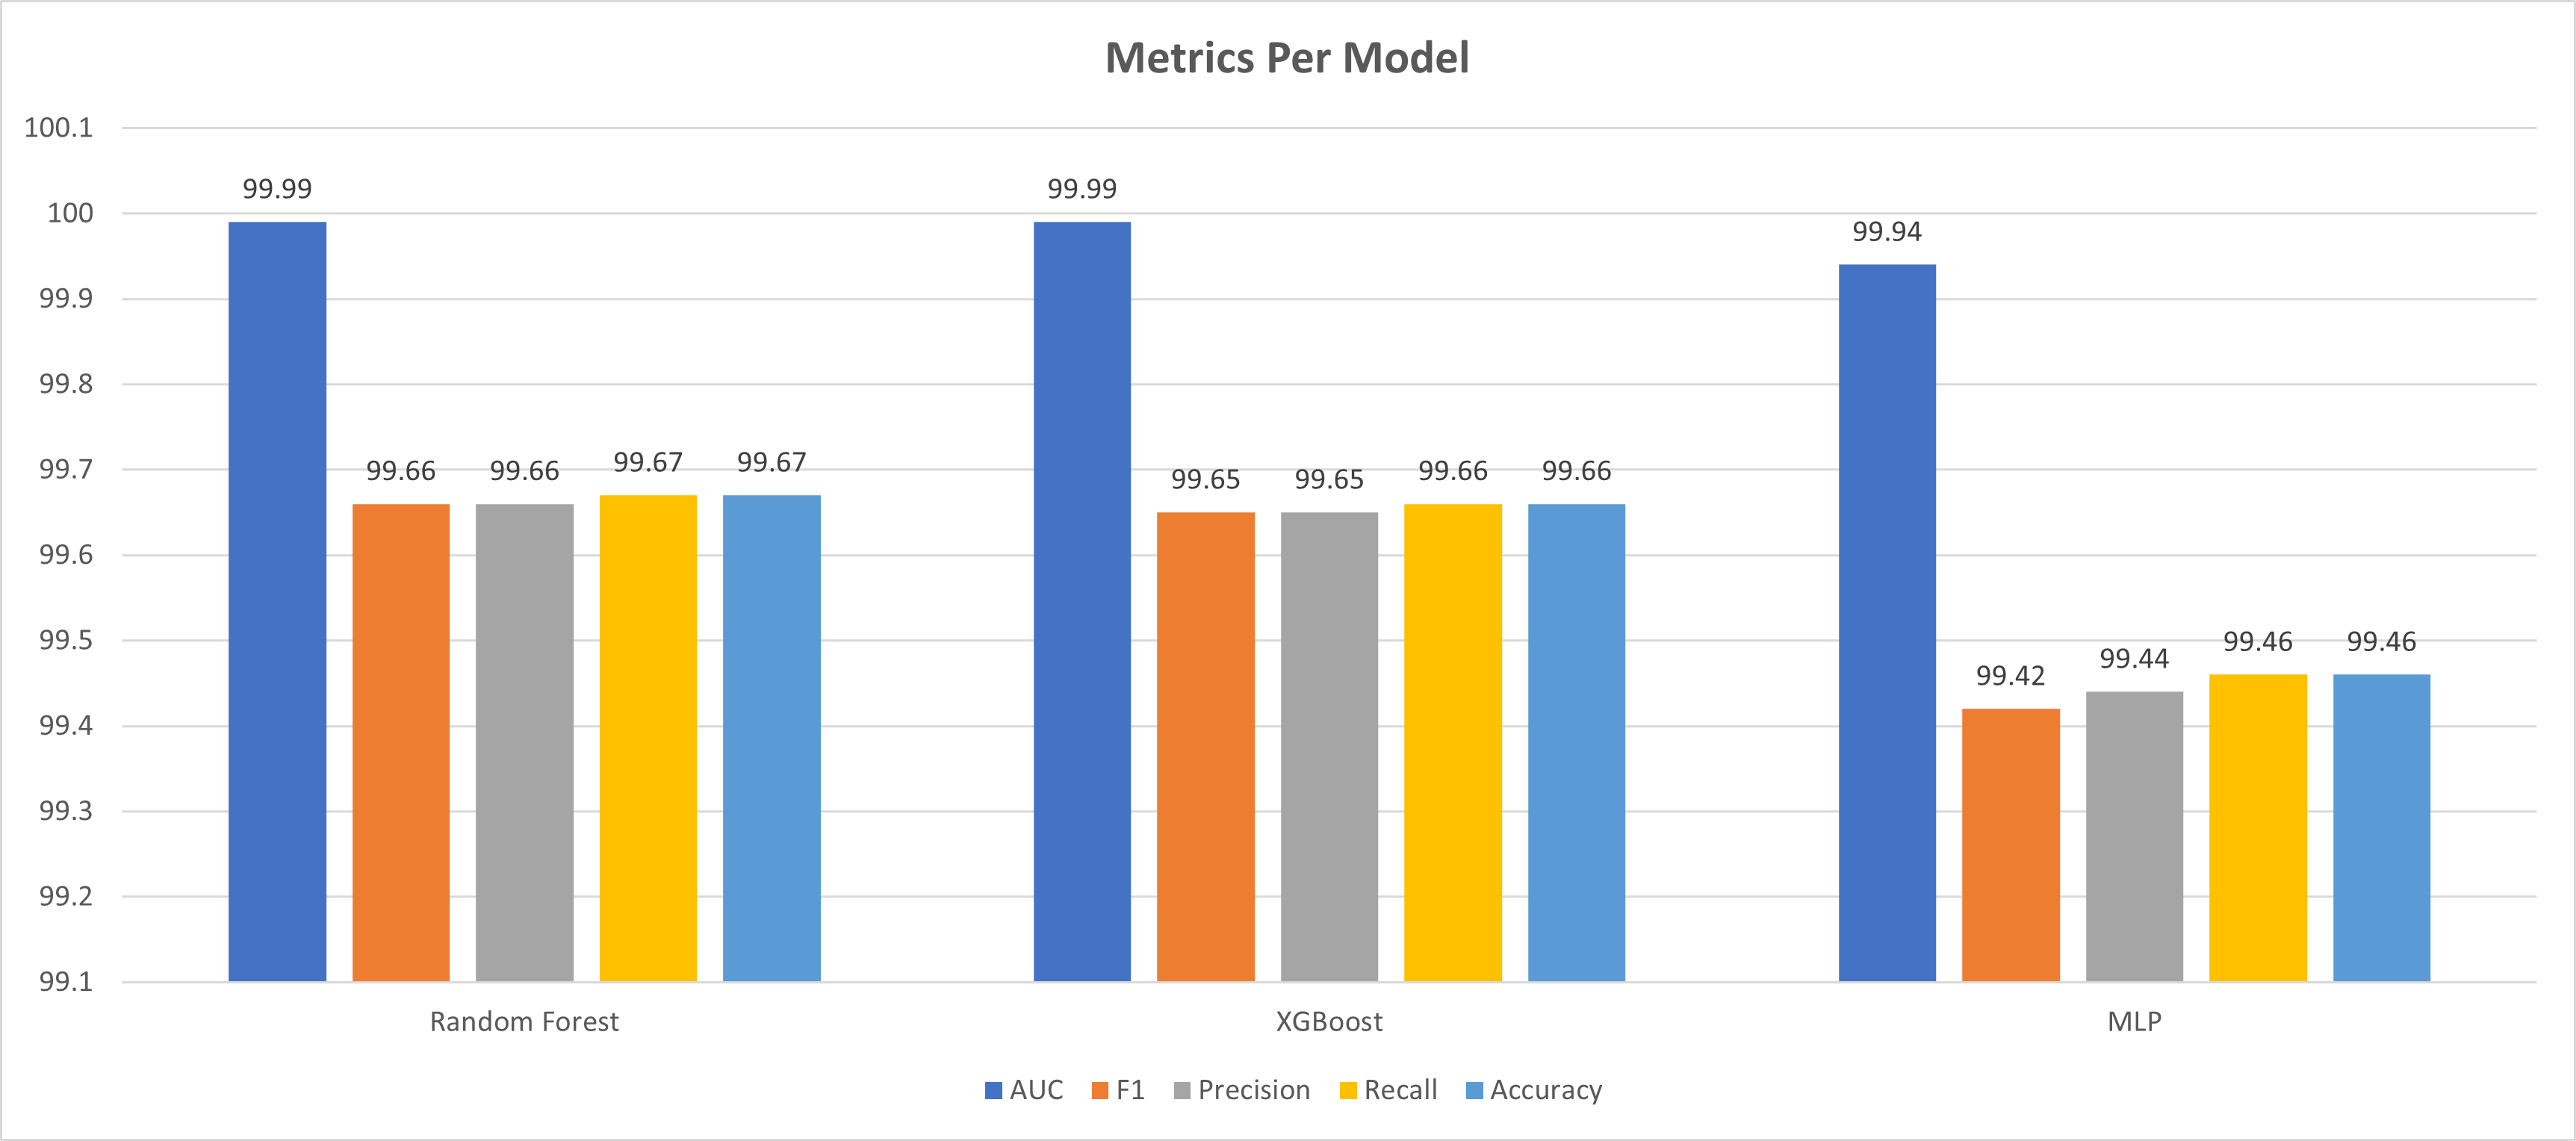
\includegraphics[width=\textwidth]{Appendices/Images/Metrics2.png}
	\caption{Metrics Grouped By Model}
  	\label{fig:model_metrics2_graph}
\end{figure}


\subsection{Feature Importance}

Random Forest and Extreme Gradient Boosting both have feature importances that can be used to interpret each model's reliance on each chosen feature. After modelling, these were examined, and the following observations were made:

\begin{itemize}
	\item Within the Random Forest Classifier, the top 4 features of importance were a range of 802.11w, non-802.11w and application layer features, such as \textit{http.request.method, ip.ttl, radiotap.dbm\_antsignal}. 
	\item Within the XGBoost Classifer, top features include more non-802.11w and application layer features such as \textit{ARP, ip.ttl, tcp.checksum.status, http.request.method, http.content\_type, dns}.
	\item Of the application layer features, the HTTP request method was of significant importance; this is proposed to be due to SSDP's attack behaviour, which relies upon the 'M\_Search' request type for a successful attack.
	\item \textit{ip.ttl} (Time to live) was consistently ranked as an important feature in the context of XGBoost and Random Forest. The time to live is an IP feature that defines the maximum number of hops the packet travels before it stops. 
\end{itemize}

\subsection{Limitations}

The experiments faced several limitations that should be considered in interpreting results and impact findings in this dissertation. Firstly, the constraints of time and computational resources hindered the ability to construct and test an exhaustive list of models, and the frequent occurrence of hardware and OS crashes negatively disrupted model training, leading to a loss in progress. In reference to the feature importance, this was explored briefly and was not fully used for feature selection or additional optimisation. 

Lastly, the iterative and exploratory approach taken for model selection and tuning could be a source of error. This may have been susceptible to undue bias or randomness, potentially leading to under-explored models. These limitations prove that although the results are high, consideration should be exercised with caution with evaluating their use for a proposed IDS. Additional research is needed to validate these models, and further work is suggested to investigate other, more complex and tuned models.

\subsection{Recommendations}

Comparing all three machine learning algorithms (see Table \ref{tab:ml-metrics} and Figures \ref{fig:model_metrics_graph}, \ref{fig:model_metrics2_graph}), experiments from this study show that the Random Forest model ran with default parameters displayed slightly better results than the other two. The XGBoost model also performed very well with similar results but had a slight increase in false positives for Botnet, Malware and SSH. The MLP model, whilst still displaying high-performance levels, appeared to struggle with classifying minority classes. The confusion matrix contains more false negatives for Botnet, Malware and SSH, suggesting it could not predict these classes accurately.

As mentioned, identifying the most optimal solution for a proposed Wireless Network Intrusion Detection System is a highly subjective challenge. The final decision ultimately depends on the performance of the models in the environment and the particular needs and focuses in the production environment. The code for each high-performing model will be in the Appendix \ref{appx: Model Code} and the project's code base.